\documentclass{article}
\usepackage{graphicx,float}
\usepackage{hyperref}
\usepackage{circuitikz}
\usepackage{pgfplotstable}
\usepackage[margin=1.0in]{geometry}
\title{Neema power system analysis software}
\author{Mohammed Elmam Abudrais}
\begin{document}
	\maketitle
	\newpage
	\tableofcontents
	\newpage
	\newpage
	\section{Introduction}
	Neema is a program for power system analysis, now it can only calculate load flow, it also include basic state estimator.
	\section{Main window}
\begin{figure}[h!]
	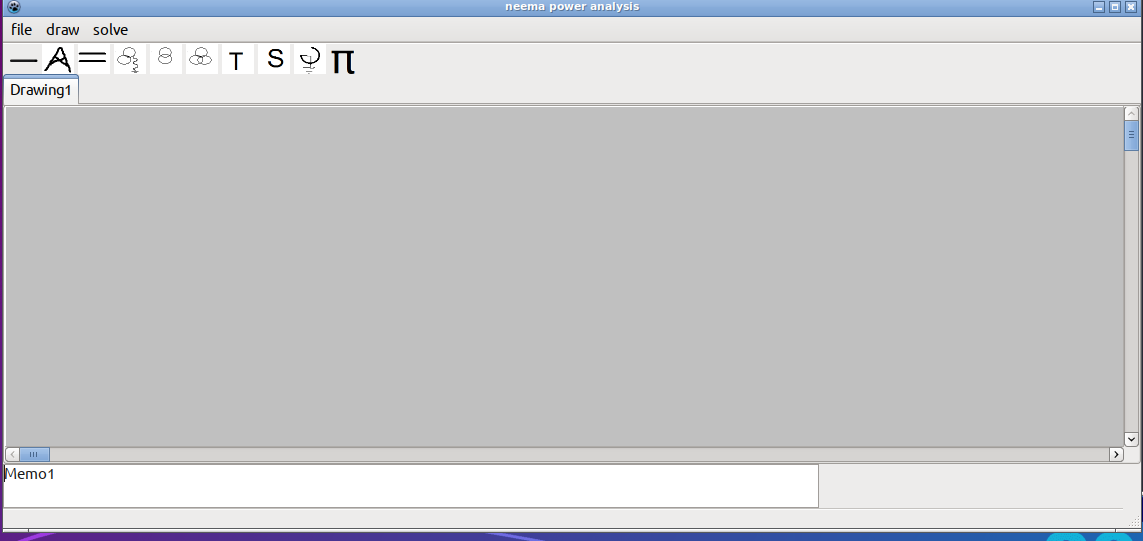
\includegraphics[width=\linewidth]{neemamain.png}
	\caption{main window}
	\label{fig:fig1}
\end{figure}
\paragraph{}the main window contain a menu, toolbar, drawing box, and message box. when you open application an empty drawing
\textbf{Drawing1} is created, you can open existing drawing using the menu \textbf{file-$>$open}
\subsection{Adding elements}
\paragraph{}
\textbf{Neema} has models for a few power system elements bus, double bus,  transmission line, 2 winding transformer, 3 winding transformer,  SVC, you can model other elements using Pi Model. every element has a button in the toolbar.
\paragraph{}
to add element to the drawing: click element button in the toolbar and then click in the drawing box, if you click a gain another element of the same type will be inserted, press \textbf{ESC} key when you finish.
\subsection{Selection}
\paragraph{}select  an elements by clicking on it, you can select more than one element, press \textbf{ESC} key to clear selection.
\subsection{Pan and move}
\paragraph{}to move an element: select it and move the mouse while pressing \textbf{shift} button. to pan (move all elements) make sure no element is selected by pressing \textbf{ESC} key, then hold \textbf{Shift} key 
and move the mouse.
\subsection{Connection}
\paragraph{}to connect elements: select two elements and press \textbf{c} key, to remove a connection select two connected elements and press \textbf{c} key. some elements can not be connected, for example you can not make connection between two buss.
\subsection{Delete}
\paragraph{}
to delete an element select it and press \textbf{Del} key.
\subsection{Setting element data}
\paragraph{}to enter element data select an element and press a window will appear, for more details about element data go to \hyperref[sec:modeldata]{model data} section.
\subsection{Search for an Element }
\paragraph{} Press \textbf{CTRL+F} to search for an element, press \textbf{F3} to find next element.
\newpage
\section{Model data}
\label{sec:modeldata}
\paragraph{} this section is about entering model data for every element type, please make sure all elements has a name, this will help in error fixing. 
\subsection{Bus model}
\paragraph{}select a bus and press \textbf{E} key the flowing dialog will appear
\begin{figure}[H]
	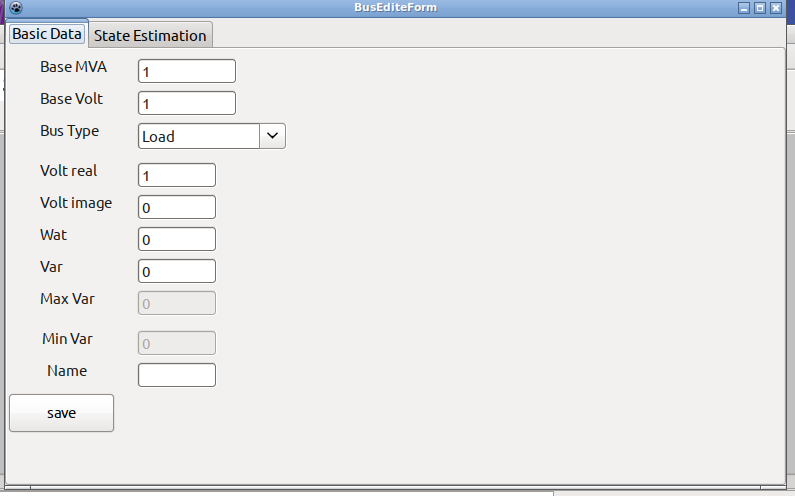
\includegraphics[width=\linewidth]{busedite.png}
	\caption{bus model window}
	\label{fig:busedite}
\end{figure}
it contain two taps: basic date, and state estimation, most field support suffix like: mw, kv, mvar. the WAT and VAR are negative for load and positive for generation, save button will check the entered data and update the bus, if an error found a message will appear and the edit box which contain the wrong data will be active.
\begin{figure}[H]
	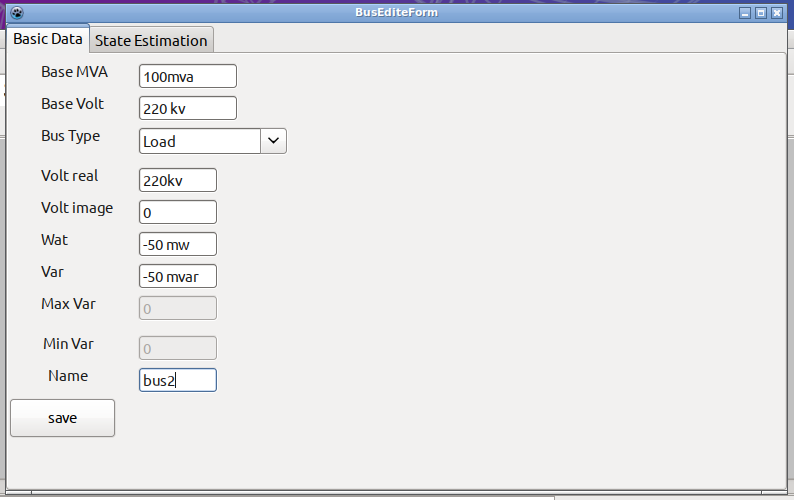
\includegraphics[width=\linewidth]{busedite2.png}
	\caption{bus model example}
	\label{fig:busediteexample}
\end{figure}
\subsection{Double bus}
\paragraph{} because \textbf{Neema} does not allow bus to bus connection, double bus partially solve this problem,but its also has it's own limitation, when bus cobbler is closed bus1 and bus2 must have type as listed below, for example if bus1 is type is slack then bus2 can not be slack or regulation.
\begin{table}[h!]
	\begin{center}
		\caption{supported bus type when Bus coupler is closed}
		\label{tab:table1}
		\begin{tabular}{c|c} % <-- Alignments: 1st column left, 2nd middle and 3rd right, with vertical lines in between
			\textbf{bus1 type} & \textbf{bus2 type}\\
			\hline
			slack & load \\
			load & load \\
			load & slack \\
			load & regulating \\
			regulating & load \\
		\end{tabular}
	\end{center}
\end{table}
\subsection{Line model}
\paragraph{}Neema use long line pi model for transmission line. 
\begin{figure}[H]
	\begin{center}
		\begin{circuitikz}
			\draw (2,0)node[ground]{}
			to[generic=$Y$](2,2)
			to[generic=$Z$](4,2)
			to[generic=$Y$](4,0)node[ground]{};
			\draw (1,2)to[short](2,2);
			\draw (4,2)to[short](5,2);
		\end{circuitikz}
		\caption{transmission line pi model}
		\label{fig:TlineModle}
	\end{center}
\end{figure}
here is an example of transmission line data:
\begin{figure}[H]
	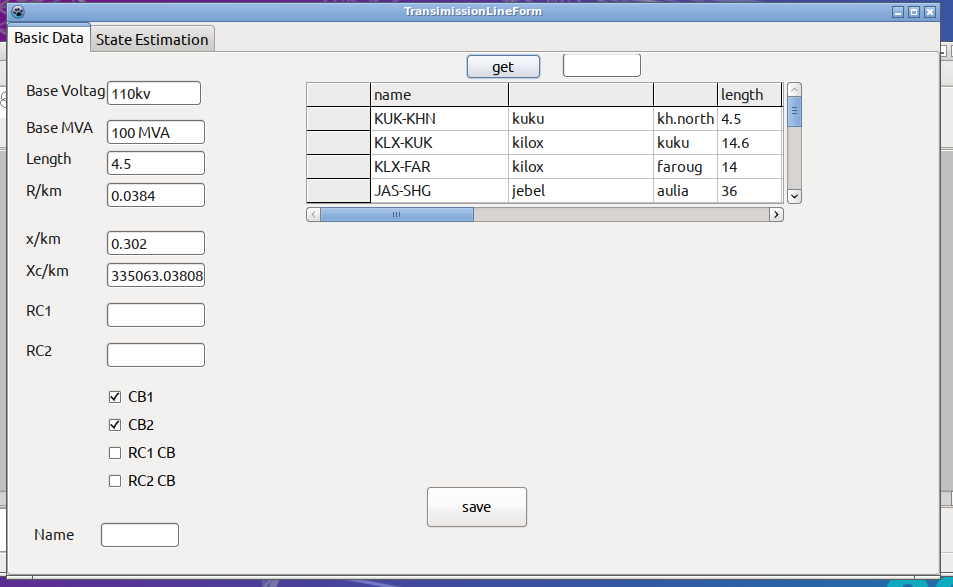
\includegraphics[width=\linewidth]{lineediteex.png}
	\caption{line mode example}
	\label{fig:lineedite}
\end{figure}
most field are self explanatory,
$X_C=1/(2\pi fc)$
\textbf{RC1} and \textbf{RC2} are reactor in line terminal in var , \textbf{CB1} and \textbf{CB2} are line circuit breakers, \textbf{RC1 CB} is reactor Circuit breakers.there is lib of common lines parameter, you can add your own data by editing LINELIB.csv file. press \textbf{Save} when you finish editing.
\subsection{Two winding transformer}
\paragraph{} \textbf{Neema} also use pi model for two winding transformer, \textbf{Neema} support transformer taps, the \textbf{R} and \textbf{X} are in per unit, the transformer breaker are either both closed or both  open.
\begin{figure}[H]
	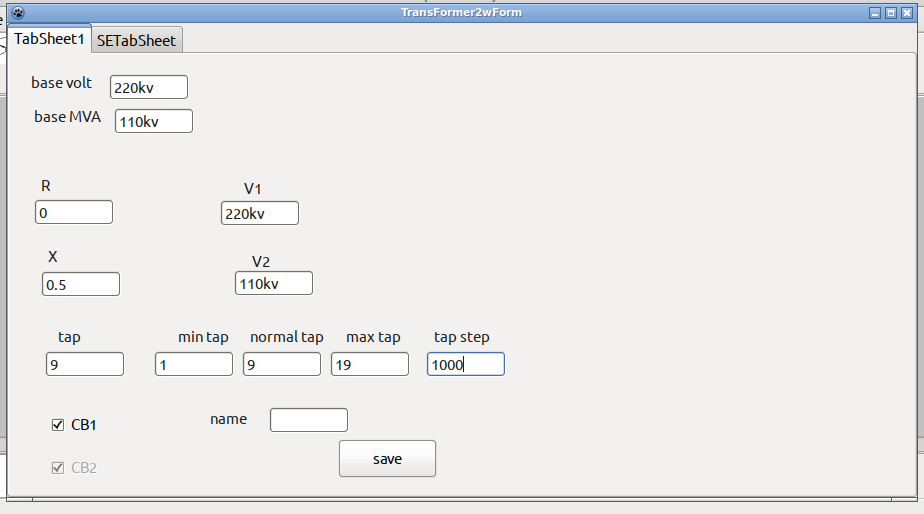
\includegraphics[width=\linewidth]{t2w.png}
	\caption{two winding transformer example}
	\label{fig:t2w}
\end{figure}
\subsection{Three winding transformer}
\begin{figure}[H]
	\begin{center}
		\begin{circuitikz}
			\draw (2,0)node[ground]{}
			to[generic=$tap$](2,2)
			to[generic=$Z1$](4,2)
			to[generic=$tap$](4,0)node[ground]{};
			\draw (7,3)
			to[generic=$Z2$](5,2)to[short](4,2);
			\draw (7,1)
			to[generic=$Z3$](5,2);
			\draw (1,2) node[above]{$primary$} to[short](2,2);
			\draw (8,3) node[above]{$secondary$} to[short](7,3);
			\draw (8,1) node[above]{$tertiary$} to[short](7,1);
		\end{circuitikz}
		\caption{3 winding transformer model}
		\label{fig:TlineModle}
	\end{center}
\end{figure}
\paragraph{} 3 winding transformer only support tap in primary side, and like two winding transformer R1, X1, R2, X2, R3, X3 are in per unit, avoid negative X value because Load flow tend to diverge with negative value,  and due limitation load flow solver not all circuit breaker position are allowed. \textbf{Neema} contain a \hyperref[sec:T3wtool]{tool} to calculate per unit impedance for three winding transformer.
\begin{figure}[H]
	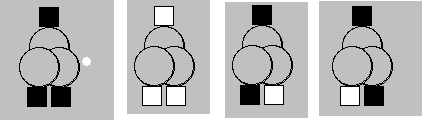
\includegraphics[width=\linewidth]{t3wcb.png}
	\caption{supported cb position,any thing else and load flow solver may not work}
	\label{fig:t2w}
\end{figure}
\subsection{3w winding transformer with shunt}
this is same as 3 winding transformer but the tertiary winding is connected to reactor. 
\subsection{Shunt}
this is a reactor or capacitor with circuit breaker, var is positive for reactor and negative for capacitor.
\begin{figure}[H]
	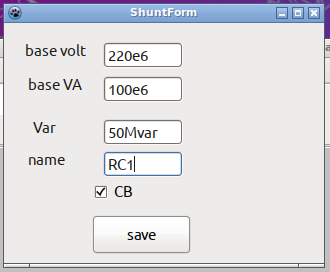
\includegraphics[width=5 cm]{shuntedit.png}
	\caption{example of shunt data}
	\label{fig:shuntex}
\end{figure}
\subsection{Solving load flow}
\paragraph{}from menu press \textbf{solve -$>$ load flow} choose start type and press \textbf{Run}, the calculated voltage will appear in the bus and the transmission line will show the MW and MVAR, you can click the menu \textbf{result-$>$load flow result} to see more details. if an error message appear please look at message box for more detail to help fixing the error.
\paragraph{} newton Raphson method need a good starting value of bus voltage to converge \textbf{Neema} provide three way to set load flow starting voltage:\begin{enumerate}
\item \textbf{flat start:} all bus start with voltage equal to 1 $pu$ except for slack and regulated bus.
\item \textbf{calculated voltages}:\textbf{Neema} will use voltage calculated by previous load flow or state estimator. 
\item \textbf{entered voltage:} \textbf{Neema} will the voltage entered by user in bus form.
\end{enumerate} 
\subsection{Result form}
\paragraph{}This form show load flow result, it can show power, var and voltages of buss transformers and transmission lines, you search for an element by entering it's name in search box,you can save the result in \textbf{csv} file.
\begin{figure}[H]
	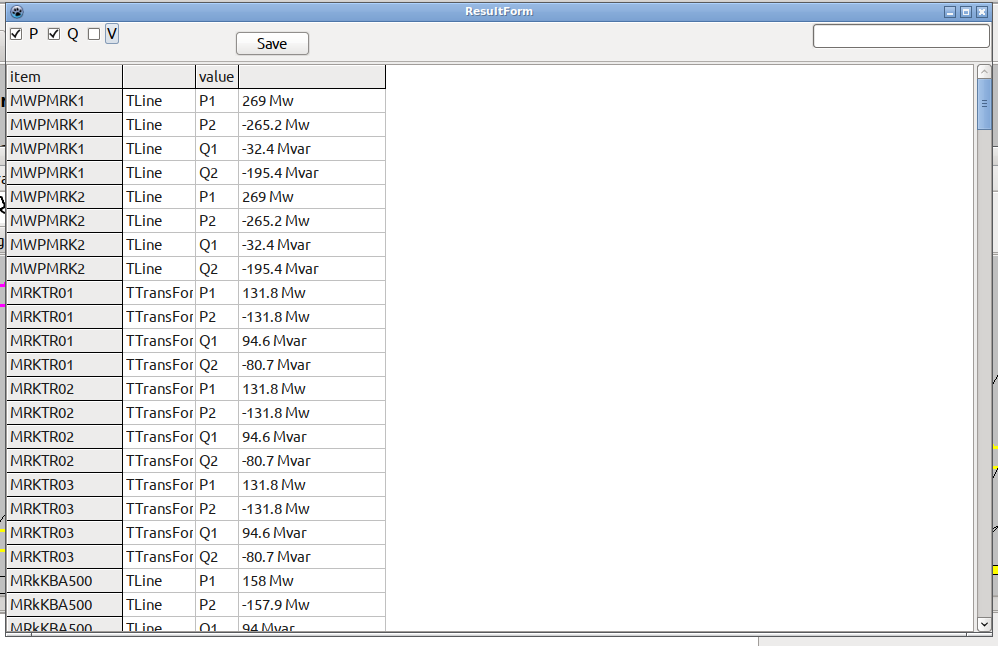
\includegraphics[width=12cm]{resultform.png}
	\caption{example of state estimation data}
	\label{fig:resultform}
\end{figure}
\newpage
\section{State estimation}
\paragraph{} state estimator calculate the state of the system($V$ and $\delta$) of every bus using available measurement \textbf{P,Q,V,I}, \textbf{Neema} state Estimator use only \textbf{p,Q} and \textbf{V}. correct status of Circuit Breaker must be entered before running the state Estimator.
\subsection{State estimator data entry}
\paragraph{} Some elements measurement like SVC,Reactor are ignored by Neema State Estimation. for other element you can enter measurement value by selecting the Element and then pressing \textbf{E} key,after that select State estimator tap, a table will appear.
\begin{figure}[H]
	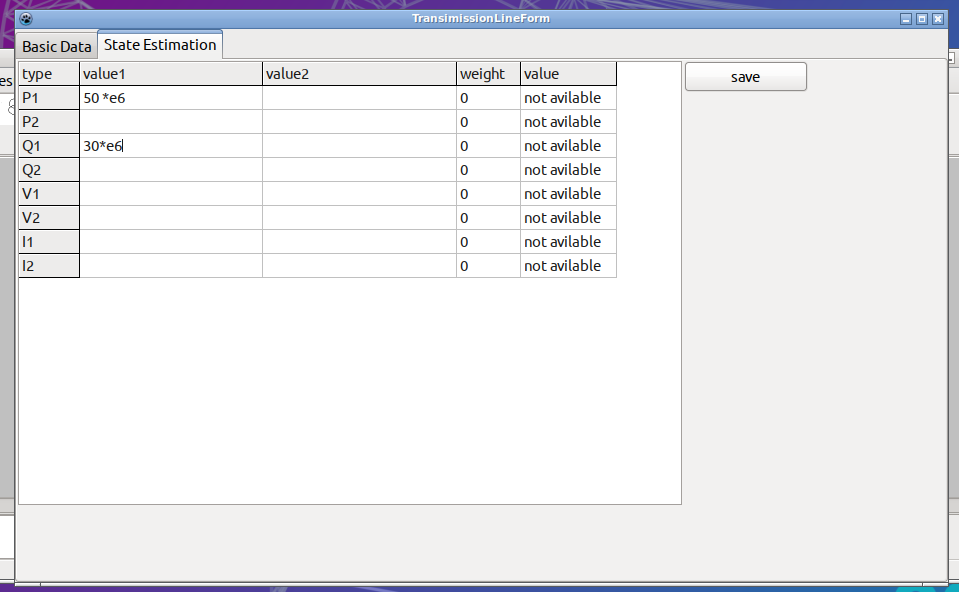
\includegraphics[width=12 cm]{linees.png}
	\caption{example of state estimation data}
	\label{fig:linesex}
\end{figure}
press save after you finish.
state estimation table do not support suffix(\textbf{MW MVAR,KV} ..etc), if the measurement value is 50 MW : it should entered as 50e6 in the table, 100KV will be 100e3, this may be supported in the next version.
\subsection{Observably}
\paragraph{}Before state Estimator start estimating an element it check if it observable, \textbf{Neema} can isolate unobservable element so you can run state estimator again. add more measurement to make element observable.
\subsection{Slack bus}
\paragraph{} Neema state estimation need slack bus voltage measurement to run, and every element element  need to have a path to slack bus to be observable.
\subsection{Runing state estimator}
\paragraph{} Run the state estimator from the menu \textbf{solve-$>$state estimate} 
\newpage
\section{Tools}
\subsection{3 winding transformer tool}
\label{sec:T3wtool}
\paragraph{} this tool calculate the per unit impedance of three winding transformer, you enter the short circuit test data of the transformer then impedance's \textbf{Z1,Z2,Z3} are calculated, fallowing are two examples, the input data are highlighted in red.
\subsubsection{Example 1}
\begin{figure}[H]
	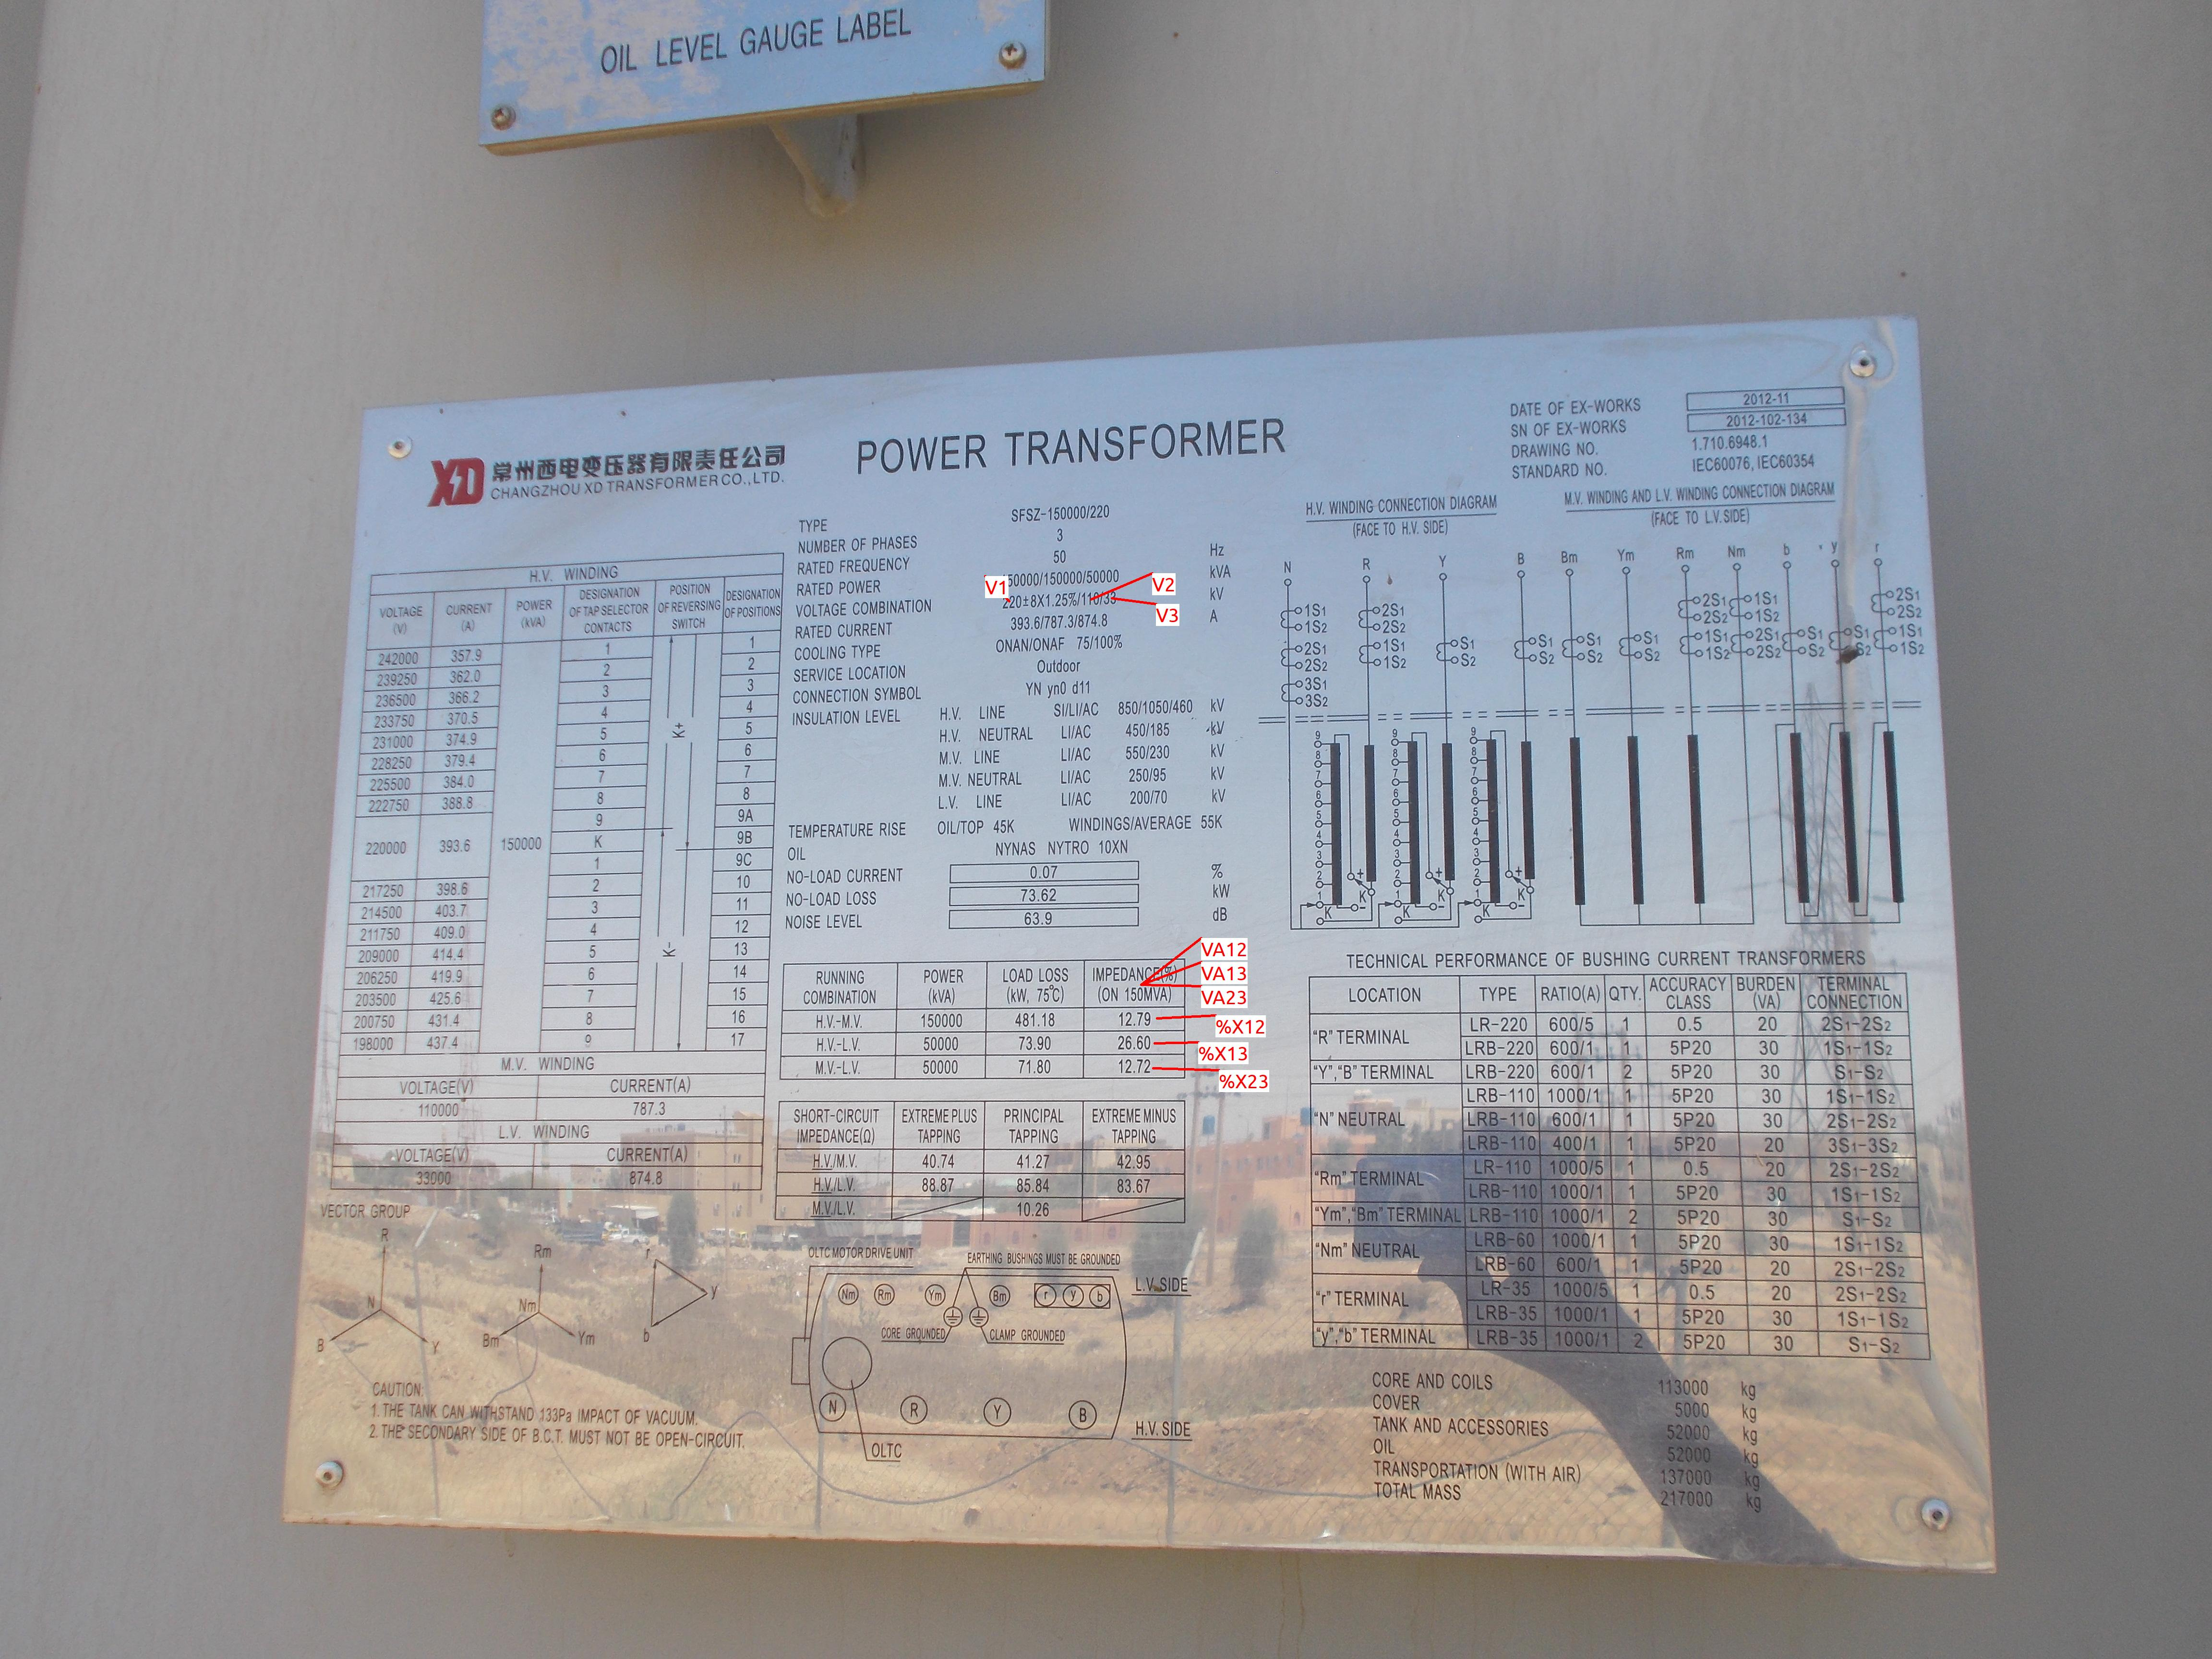
\includegraphics[width=\linewidth]{MHDTR01.jpg}
	\caption{transformer 1 name plate }
	\label{fig:TR01}
\end{figure}
\begin{figure}[H]
	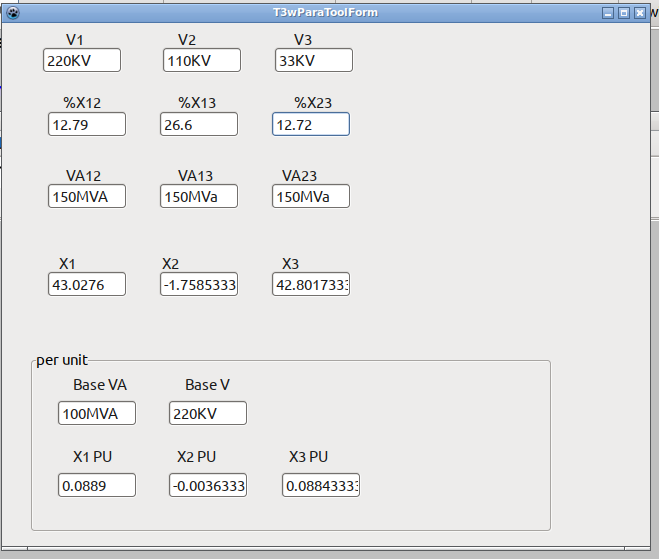
\includegraphics[width=\linewidth]{MHDTR01Tool.png}
	\caption{transformer 1 data in 3w transformer toll }
	\label{fig:TR01}
\end{figure}
	figure 13 give an example of how to enter the data from name plate fig 12.
	\textbf{V1, V2, V3, \%X12 , \%X13, \%X23 , VA12, VA13, VA23} are obtained from name plate, \textbf{Base VA} is the base VA for the drawing, \textbf{Base V} is the base voltage of the bus bar connected to the primary side of the transformer, \textbf{Neema} transformer model require impedance per unit value \textbf{X1 PU, X2 PU, X3 PU}, in this example the calculated \textbf{X2 PU}=-0.0031 you should multiply by -1, as mentioned earlier negative impedance tend make  load flow diverge, replacing -0.0031 by 0.0031  will introduce a very small error in the solution.
	\newpage
\subsubsection{Example 2}
\begin{figure}[H]
	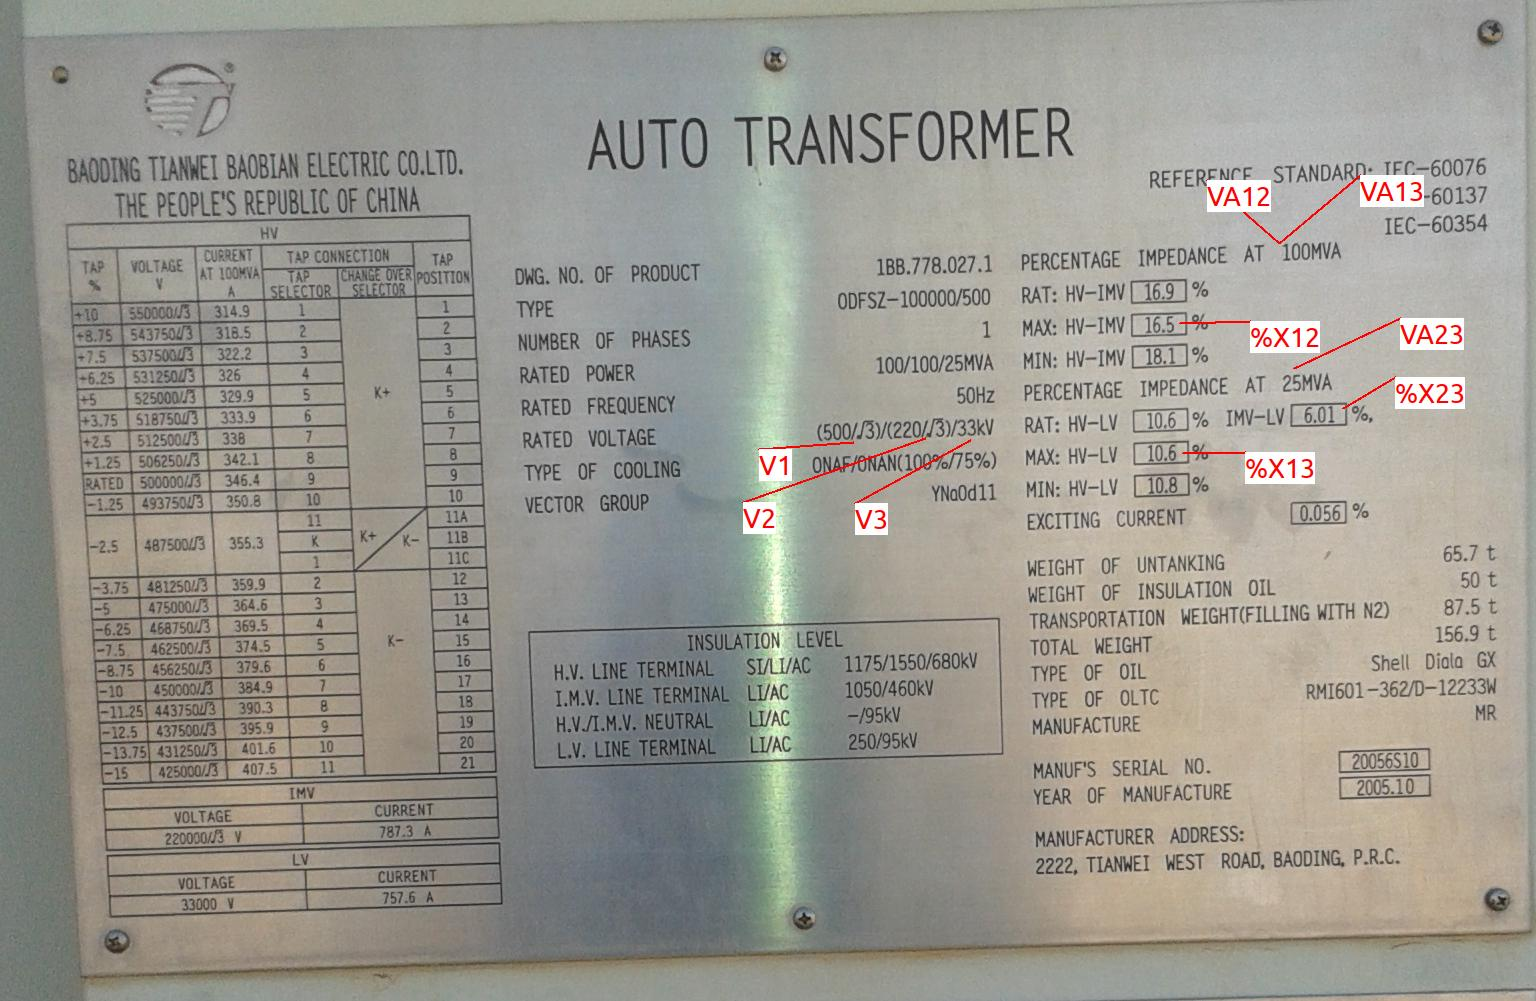
\includegraphics[width=\linewidth]{MRKTR01.jpg}
	\caption{transformer 2 name plate }
	\label{fig:TR02}
\end{figure}
\begin{figure}[H]
	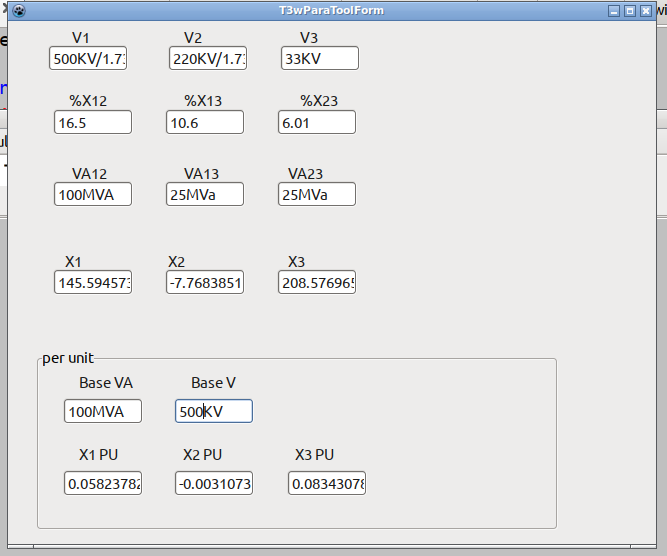
\includegraphics[width=\linewidth]{MRKTR01tool.png}
	\caption{transformer 2 data in 3w transformer toll }
	\label{fig:TR02tool}
\end{figure}
\end{document} 